\documentclass[tikz,border=4pt]{standalone}
\usepackage{amsmath}
\begin{document}
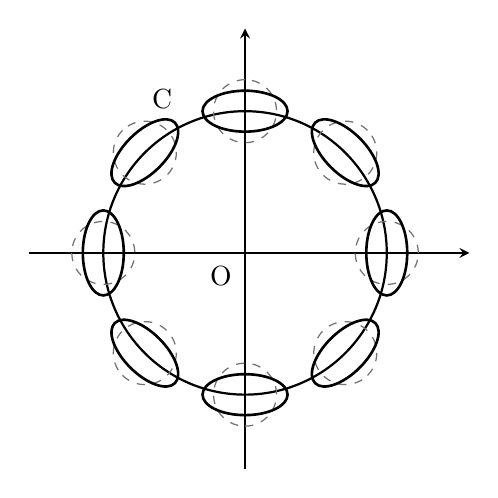
\begin{tikzpicture}[>=stealth, thick, scale=1.0]
  % Coordinate axes
  \draw[->, line width=0.6pt] (-2.75, 0) -- (2.85, 0);
  \draw[->, line width=0.6pt] (0, -2.75) -- (0, 2.85);
  \node[below left] at (-0.04, -0.04) {$\mathrm{O}$};

  % Unit circle C (radius R = 1.8)
  \draw[line width=0.8pt] (0, 0) circle (1.8);
  \node[above left] at (115:1.88) {$\mathrm{C}$};

  % Original 8 dashed circles (r = 0.40) and deformed solid ellipses
  % Radial axis scaled by 1 - gamma = 0.65 -> a_r = 0.26
  % Tangential axis scaled by 1 + gamma = 1.35 -> a_t = 0.54
  \foreach \ang in {0, 45, 90, 135, 180, 225, 270, 315} {
    \begin{scope}[shift={(\ang:1.8)}, rotate=\ang]
      \draw[dashed, line width=0.45pt, black!55] (0, 0) circle (0.40);
      \draw[line width=0.95pt] (0, 0) ellipse[x radius=0.26, y radius=0.54];
    \end{scope}
  }
\end{tikzpicture}
\end{document}
